\section{Netze}

\GrayBox{Netze sind alle Einrichtungen zusammen (Freileitungen, Kabel, Umspannanlagen und Schaltanlagen, die zur Übertragung und Verteilung der elektrischen Energie notwendig sind) \newline\newline Übertragen elektrischer Energie mit Gleichstrom, Wechselstrom oder Drehstrom – wird nach Wirtschaftlichkeit gewählt.}

\begin{itemize}
    \item[\textbf{Stromnetz:}] Netzwerk aus Stromleitungen (Freileitungen und Erdkabeln) und Einrichtungen (Schalt- und Umspannwerke) sowie Kraftwerke und Verbraucher
    \item[\textbf{Bordnetze:}] Stromnetz in Fahr- und Flugzeugen
\end{itemize}

\vspace{1em}

\textit{Die österreichische Stromversorgen gehört mit einer Verfügbarkeit von 99,9\% zu den sichersten der Welt.}

Mehr Investition in die Netze und Infrastruktur ist notwendig, da es durch den Ausbau der erneuerbaren Energie zu Erzeugungsschwankungen kommt.

\subsection{Struktur von Versorgungsnetzen}

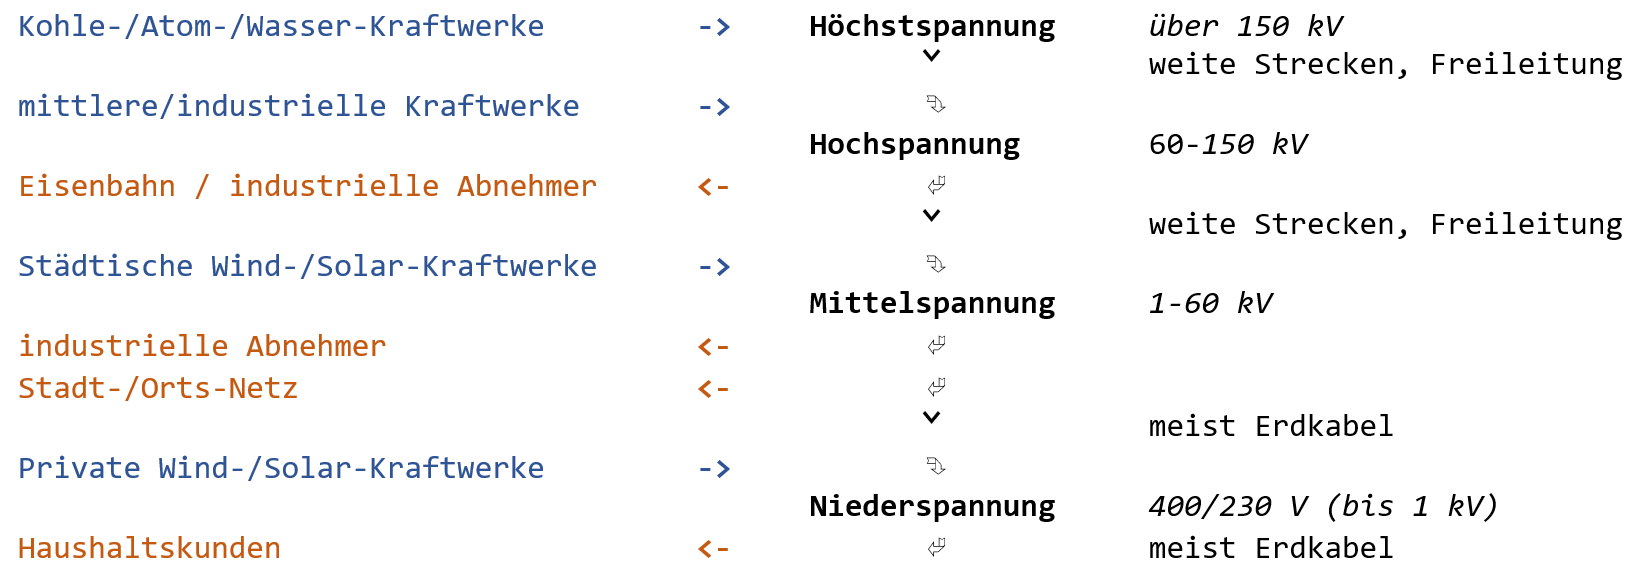
\includegraphics[width=\textwidth]{images/01-Netze/StrukturVersorgungsnetze.png}

\subsection{Eigenschaften von Versorgungsnetzen}

\begin{itemize}
    \item \textbf{Höchstspannungsnetz} \textit{(meist 220 und 380 kV)}
    \newline Dient als Verbundnetz für den überregionalen und internationalen Austausch, sowie zur regionalen Übertragung von großen Kraftwerken zu den unteren Netzen.
    \item \textbf{Hochspannungsnetz} \textit{(meist 110 kV)}
    \newline Es speisen mittlere und kleinere Kraftwerke ein und dient zur Übertragung und Verteilung. – Primärverteilung
    \item \textbf{Mittelspannungsnetze} \textit{(meist 10 und 30 kV)}
    \newline Es werden viele Sondervertragskunden versorg und in die Niederspannung-Ortsnetze gespeist. – Sekundärverteilung
    \item \textbf{Niederspannungsnetze} \textit{(400/230 V)}
    \newline Tarifkunden der öffentlichen Energieversorgung werden versorgt.
    \item \textbf{Industrienetze} \textit{(meist 6 kV)}
    \newline Hohe Versorgungszuverlässigkeit und teilweise sind Abnehmer mit hohen Netzrückwirkungen (z.B. große Motoren) angeschlossen.
\end{itemize}

\vspace{1em}

\GrayBox{Die verschiedenen Spannungsebenen werden meist über Transformatoren miteinander verbunden}

\vspace{2em}

\begin{itemize}
    \item[\textbf{Übertragungsnetzbetreiber:}] Betrieb der Stromnetze, aus denen das Verbundnetz besteht. In Österreich nur Austrian Power Grid AG (APG).
    \item[\textbf{Verbundnetzbetreiber:}] Betrieb der Stromnetze, aus denen die Hochspannungsebene besteht.
\end{itemize}

%\begin{noindent}
\begin{markdown}

Es wird zwischen **unvermaschte** und **vermaschte** Netze unterschieden:

\vspace{1em}

## Unvermaschte Netze

### Stern-(Strahlen) Netz

**Aufbau**

Energiefluss geht vom Speisepunkt aus strahlenförmig in mehrere Leitungsstrecken.

**Vorteile**

- Einfache Netzüberwachung und Planung
- Kleine Kurzschlussströme

**Nachteile**

- Spannungsabfall zunehmend zum Leitungsende
- Geringe Versorgungssicherheit _(Bei Störabschaltung werden alle Verbraucher getrennt)_

Kommt z.B.: bei Neubaugebieten, abgelegenen Verbraucher, Hochhäuser oder Gewerbebetrieben in Einsatz

\begin{figure}[H]
    \centering
    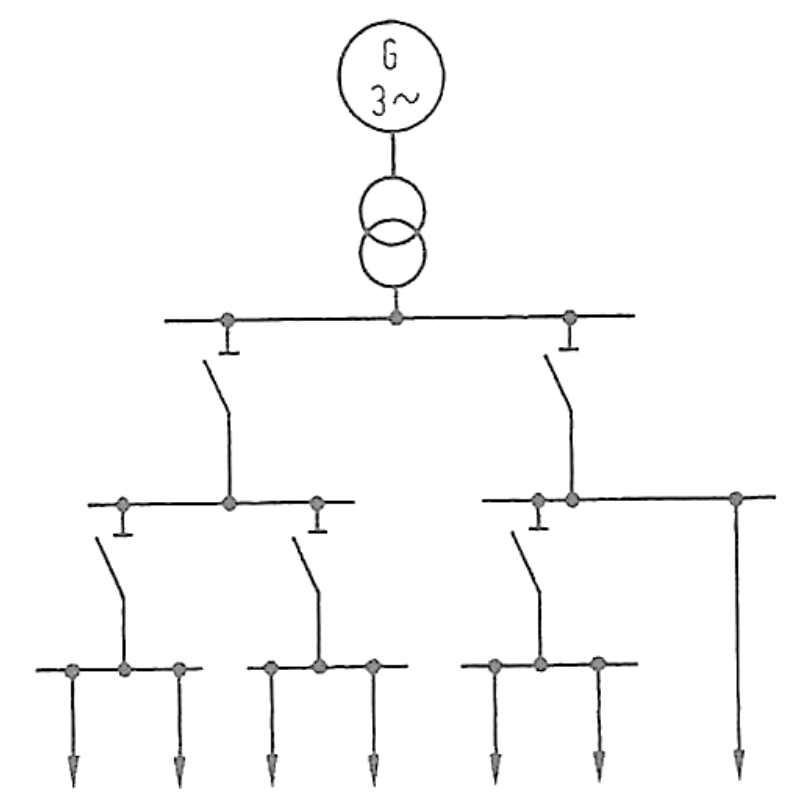
\includegraphics[width=0.5\textwidth]{./images/01-Netze/Sternnetz.png}
    \caption[Aufbau eines Stern-(Strahlen) Netzes]{Aufbau eines Sternnetzes}
\end{figure}

\newpage

## Vermaschte Netze

### Ringnetz

**Aufbau**

Energiefluss geht vom Speisepunkt aus parallel in zwei Ringstrecken, deren enden über Kuppelschalter verbunden sind.

**Vorteile**

- Kuppelschalter ermöglicht betrieb als Ringnetz oder Strahlennetz
- Einspeisung aus zwei verschiedenen Quellen möglich
- Auftrennung bei Störungen durch Schaltmöglichkeiten

Kommt in der öffentlichen Energieversorgung z.B.: zur Speisung von Ortsnetz-Transformatoren aus einem Mittelspannungsnetz in Einsatz.

\begin{figure}[H]
    \centering
    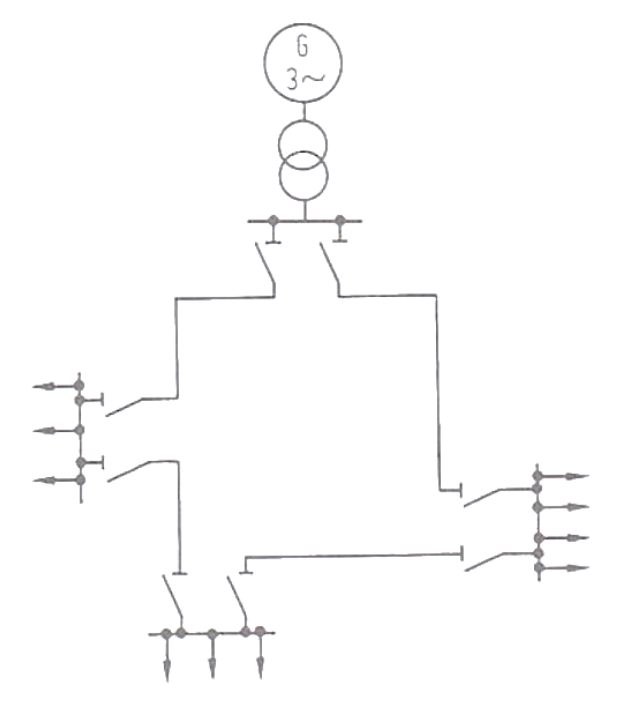
\includegraphics[width=0.4\textwidth]{./images/01-Netze/Ringnetz.png}
    \caption[Aufbau eines Ringnetzes]{Aufbau eines Ringnetzes}
\end{figure}

### Maschennetz

\begin{wrapfigure}{r}{0.4\textwidth}
    \centering
    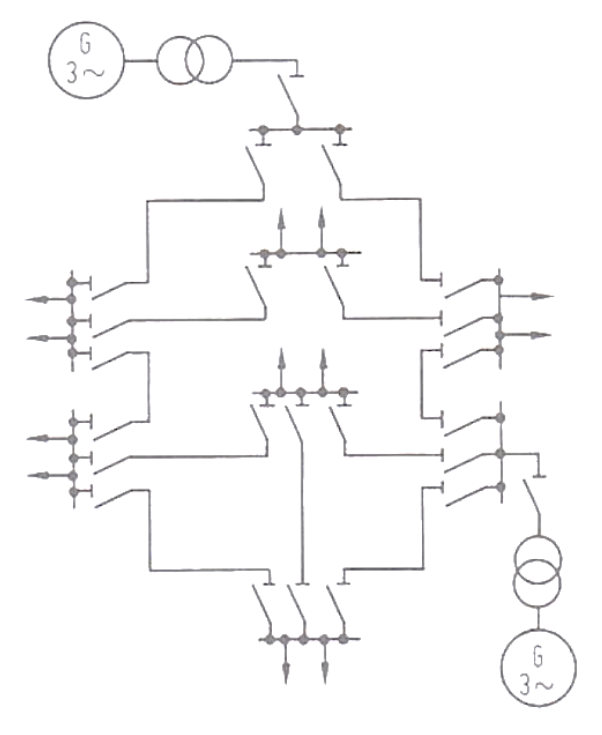
\includegraphics[width=0.3\textwidth]{./images/01-Netze/Maschennetz.png}
    \caption[Aufbau eines Maschennetzes]{Aufbau eines Maschennetzes}
\end{wrapfigure}

**Aufbau**

Ringnetz mit Querverbindungen.

Je enger die Vermaschungen, desto geringer die Spannungsabfälle und desto größer wird die Versorgungssicherheit. Andererseits vergrößern sich die Kurzschlussströme und die Schwierigkeiten bei der Überwachung.

**Vorteile**

- Geringer Spannungsabfall
- Geringe Leitungsverluste
- Hohe Versorgungssicherheit

**Nachteile**

- Großer Kurzschlussstrom
- Aufwendige Schaltanlage
- Hohe Anforderungen an den Netzschutz

Kommt bei allen Spannungsebenen der öffentlichen Energieversorgung und z.B.: bei Niederspannungs-, Mittelspannungs- und Hochspannungsnetze in Einsatz. _(In der Höchstspannungsebene erfolgt der Betrieb bei einem bestimmten Vermaschungsgrad)_

\newpage

## Doppelstrahlen-(Industrie) Netz - Sonderfall

**Eigenschaften**

- Zwei Einspeisepunkte aus der 110kV-Ebene
- Jede Spannungsebene kann bei den Knotenpunkten über unabhängige Einspeisungen versorgt werden.
- Die Drosselspulen dienen, zur Begrenzung der Kurzschlussströme

**20 kV-Mittelspannungsebene**

- Besteht aus zwei Netzgruppen, welche über Drosselspulen gekuppelt sind.
- In jede Netzgruppe speist ein Generator ein.

**6 kV-Ebene**

- Besteht aus zwei Netzgruppen, welche über Drosselspulen gekuppelt sind.
- Betreibt Abnehmer mit hohen Leistungen (z.B.: große Motoren)

**400 V-Niederspannungsebene**

- Betreibt Abnehmer mit kleineren Leistungen

\begin{figure}[H]
    \centering
    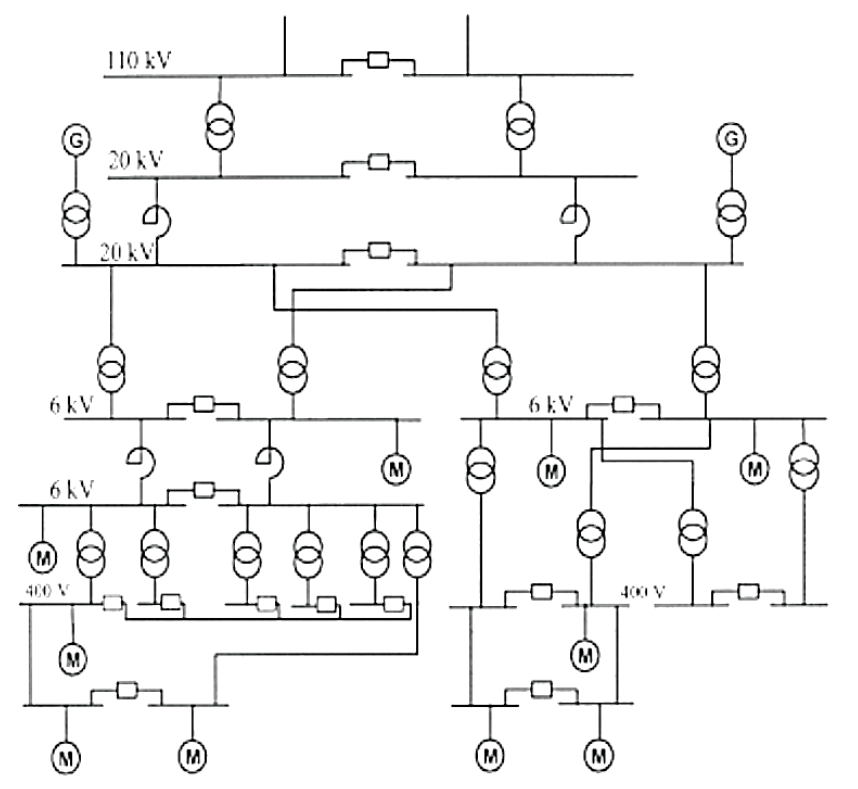
\includegraphics[width=0.6\textwidth]{./images/01-Netze/Doppelstrahlennetz.png}
    \caption[Aufbau eines Doppelstrahlennetzes]{Aufbau eines Doppelstrahlennetzes}
\end{figure}

## Grundsätze der Netzplanung

**Forderungen**

- Einfacher Netzaufbau
- Standardisierte Betriebsmittel
- Große Versorgungssicherheit
- Kleine Verluste
- Günstige Erweiterungsmöglichkeiten

Meistens wird das Netz als vermaschtes Netz (Ring-/Maschennetz) erstellt, welches aus mehrere unvermaschten (Strahlennetz) Zweige besteht:

- Das Maschennetz bietet gute Erweiterungsmöglichkeiten.
- Durch das Strahlennetz können fehlerhafte Elemente herausgetrennt werden und die Verbraucher können durch zuschalten eines anderen Maschenzweigs weiter versorgt werden.

\end{markdown}